
\chapter{Introduzione}


\section{TCP/IP e modello a strati}

% https://en.wikipedia.org/wiki/Internet_protocol_suite
% https://it.wikipedia.org/wiki/Modello_OSI
% https://datatracker.ietf.org/doc/html/rfc1122
% https://datatracker.ietf.org/doc/html/rfc791
% https://datatracker.ietf.org/doc/html/rfc791#section-2.1
% https://datatracker.ietf.org/doc/html/rfc791#section-2.2


%%% \cite https://datatracker.ietf.org/doc/html/rfc1122#section-1
\begin{comment}
An Internet communication system consists of interconnected packet networks supporting communication among host computers using the Internet protocols.  The networks are interconnected using packet-switching computers called "gateways" or "IP routers" by the Internet community, and "Intermediate Systems" by the OSI world [INTRO:13].

After looking at the major milestones in the history of the Internet, let's take a closer look into the current architectural design of the Internet.

Connecting hosts running the same applications but located in different types of networks. A computer network is a complex system that is built on top of multiple components. These components can vary in technologies making up different types of networks that offer different types of applications. For example in the figure below, we have two BitTorrent clients that communicate even though they are using very different networks/technologies (Wifi vs Ethernet). So, how do these technologies and components interconnect and come together to meet the needs of each application? The designers of the network protocols provide structure to the network architecture by organizing the protocols into layers.
\end{comment}


% ok
Internet costituisce la piu' grande rete di comunicazione al mondo, con piu' di 5 miliardi\cite{owidinternet} di dispositivi connessi nello stesso momento. Eppure la sua architettura di base e' relativamente semplice, tutto e' incentrato su un set di protocolli e i dispositivi che li implementano.

% nop
Per mantenere la complessita' bassa i protocolli sono raccolti in 4/8 strati, in base al modello che si sceglie di seguire (ISO/OSI vs TCP/IP).

\begin{comment}
Un sistema di comunicazione Internet consiste in un interconnessione tra reti di pacchetti, che supportano la comunicazione tra hosts usando una suite di protocolli.

L'obbiettivo di Internet è quello di collegare hosts attraverso una rete geografica, indipendentemente dalla distanza o da quali mezzi fisici vengano usati per trasferire i dati. Deve quindi essere in grado di gestire una grande varietà di applicazioni, tipi di rete e mezzi di trasmissione. Per garantire la flessibilità necessaria e non aggiungere troppa complessità, l'architettura di Internet è sta suddivisa in alcuni strati.

\end{comment}

\subsection{Internet Protocol Suite}

%%  Internet Protocol Suite
%%
%%    To communicate using the Internet system, a host must implement
%%    the layered set of protocols comprising the Internet protocol
%%    suite.  A host typically must implement at least one protocol
%%    from each layer.

Per comunicare su Internet, gli Host devono implementare un set di protocolli che costituiscono l'\it{Internet protocol suite} \cite{RFC_1122}. I protocolli si suddividono in strati logici che li raggruppano in 4 categorie, ogni Host deve implementare almeno un protocollo per ogni strato.

\begin{figure}[H]
    \centering
    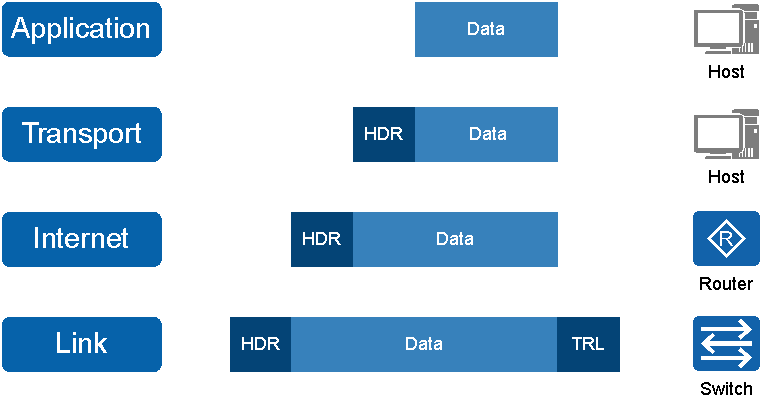
\includegraphics[width=0.8\textwidth]{immagini/diag2-modello_a_strati}
    \caption{Rappresentazione degli strati del modello TCP/Ip con relativo incapsulamento e dispositivo di dominio}
    \label{fig:modello-a-strati}
\end{figure}



%%    The protocol layers used in the Internet architecture are as
%%    follows [INTRO:4]:
Vediamo una breve descrizione dei layer e delle loro funzioni:

\begin{enumerate} % \cite https://datatracker.ietf.org/doc/html/rfc1122#section-1
    \item[layer 4:] \textbf{Application}: Il livello applicazione è il layer pi\`u alto dell'\it{Internet protocol suite}, i protocolli di questo livello si suddividono in protocolli utente e di supporto. \newline
    I protocolli utente espongono un servizio direttamente all'utente finale, alcuni esempi sono: \href{https://en.wikipedia.org/wiki/Hypertext_Transfer_Protocol}{http}, \href{https://en.wikipedia.org/wiki/File_Transfer_Protocol}{ftp}, \href{https://en.wikipedia.org/wiki/Secure_Shell}{ssh}, etc. \newline 
    % TODO da riscrivere!!
    I protocolli di supporto forniscono alcune funzionalità di supporto per il funzionamento della rete, alcuni esempi sono: \href{https://en.wikipedia.org/wiki/Domain_Name_System}{DNS}, \href{https://en.wikipedia.org/wiki/Simple_Network_Management_Protocol}{SNMP} etc.

%%        The application layer is the top layer of the Internet
%%        protocol suite.  The Internet suite does not further
%%        subdivide the application layer, although some of the
%%        Internet application layer protocols do contain some
%%        internal sub-layering.  The application layer of the
%%        Internet suite essentially combines the functions of the
%%        top two layers -- Presentation and Application -- of the
%%        OSI reference model.
%%
%%        We distinguish two categories of application layer
%%        protocols:  user protocols that provide service directly
%%        to users, and support protocols that provide common system
%%        functions.  Requirements for user and support protocols
%%        will be found in the companion RFC [INTRO:1].
%%
%%        The most common Internet user protocols are:
%%
%%        o  Telnet (remote login)
%%        o  FTP    (file transfer)
%%        o  SMTP   (electronic mail delivery)
%%
%%        There are a number of other standardized user protocols
%%        [INTRO:4] and many private user protocols.
%%
%%        Support protocols, used for host name mapping, booting,
%%        and management, include SNMP, BOOTP, RARP, and the Domain
%%        Name System (DNS) protocols.


    \item[layer 3:] \textbf{Transport}: Il livello di trasporto fornisce una comunicazione end-to-end tra per le applicazioni, infatti in generale il campo data del livello di trasporto non viene letto da nessuno se non l'applicazione di sorgente e destinazione. I protocolli principali di questo livello sono TCP e UDP: il \href{https://en.wikipedia.org/wiki/Transmission_Control_Protocol}{TCP} è connection-oriented e fornisce alta affidabilità; mentre l'\href{https://en.wikipedia.org/wiki/User_Datagram_Protocol}{UDP} è connection-less, quindi ogni inaffidabilità della rete deve essere gestita a livello applicazione.
    
%%        The transport layer provides end-to-end communication
%%        services for applications.  There are two primary
%%        transport layer protocols at present:
%%
%%        o Transmission Control Protocol (TCP)
%%        o User Datagram Protocol (UDP)
%%
%%        TCP is a reliable connection-oriented transport service
%%        that provides end-to-end reliability, resequencing, and
%%        flow control.  UDP is a connectionless ("datagram")
%%        transport service.
%%
%%        Other transport protocols have been developed by the
%%        research community, and the set of official Internet
%%        transport protocols may be expanded in the future.
%%
%%        Transport layer protocols are discussed in Chapter 4.

    % TODO da rivedere
    \item[layer 2:] \textbf{Internet}: Tutti i protocolli di trasporto usano il protocollo Internet (IP) per portare i dati dall'host sorgente alla destinazione. Al contrario dei protocolli di livello trasporto il protocollo IP non è end-to-end, quindi è intrinsecamente di tipo connection-less, non fornisce quindi nessuna garanzia che il pacchetto arrivi a destinazione, o arrivi danneggiato o duplicato. I layer sopra al livello IP sono responsabili di mantenere l'affidabilità dei servizi quando essa è richiesta. Di questo layer fanno parte i protocolli \href{https://en.wikipedia.org/wiki/Internet_Protocol}{IP}, \href{https://en.wikipedia.org/wiki/Internet_Control_Message_Protocol}{ICMP}, etc.
    
%%        All Internet transport protocols use the Internet Protocol
%%        (IP) to carry data from source host to destination host.
%%        IP is a connectionless or datagram internetwork service,
%%        providing no end-to-end delivery guarantees. Thus, IP
%%        datagrams may arrive at the destination host damaged,
%%        duplicated, out of order, or not at all.  The layers above
%%        IP are responsible for reliable delivery service when it
%%        is required.  The IP protocol includes provision for
%%        addressing, type-of-service specification, fragmentation
%%        and reassembly, and security information.
%%
%%        The datagram or connectionless nature of the IP protocol
%%        is a fundamental and characteristic feature of the
%%        Internet architecture.  Internet IP was the model for the
%%        OSI Connectionless Network Protocol [INTRO:12].
%%
%%        ICMP is a control protocol that is considered to be an
%%        integral part of IP, although it is architecturally
%%        layered upon IP, i.e., it uses IP to carry its data end-
%%        to-end just as a transport protocol like TCP or UDP does.
%%        ICMP provides error reporting, congestion reporting, and
%%        first-hop gateway redirection.
%%
%%        IGMP is an Internet layer protocol used for establishing
%%        dynamic host groups for IP multicasting.
%%
%%        The Internet layer protocols IP, ICMP, and IGMP are
%%        discussed in Chapter 3.

    % TODO da rivedere
    \item[layer 1:] \textbf{Link}: È il layer più vicino al mezzo fisico su cui viaggiano i dati, ogni host deve implementare il protocollo usato per la specifica interfaccia che usa. Ad esempio un'host con un'interfaccia Ethernet deve implementare i protocolli \it{Ethernet II} e \it{IEEE 802.3}.
    
%%        To communicate on its directly-connected network, a host
%%        must implement the communication protocol used to
%%        interface to that network.  We call this a link layer or
%%        media-access layer protocol.
%%
%%        There is a wide variety of link layer protocols,
%%        corresponding to the many different types of networks.
%%        See Chapter 2.

\end{enumerate}

Possiamo vedere a cosa corrisponde in pratica con una cattura di un pacchetto eseguita con \it{Wireshark}:

\begin{bashcode}{Wireshark}{code:tls-wireshark}
1 > Frame 43408: 93 bytes on wire (744 bits), 93 bytes captured (744 bits) on interface wlp5s0, id 0
1 > Ethernet II, Src: IntelCor_eb:91:5f (cc:d9:ac:eb:91:5f), Dst: HuaweiDe_27:a9:24 (0c:e4:a0:27:a9:24)
2 > Internet Protocol Version 4, Src: 192.168.8.119, Dst: 142.250.180.174
3 > Transmission Control Protocol, Src Port: 36354, Dst Port: 443, Seq: 36720, Ack: 13639, Len: 39
4 > Transport Layer Security
     > TLSv1.3 Record Layer: Application Data Protocol: http-over-tls
             Opaque Type: Application Data (23)
             Version: TLS 1.2 (0x0303)
             Length: 34
             Encrypted Application Data: 389bf9516cce567d0d90ef62ba2a87376091fedb7f66f3b9e60e45a39376b1ae667a
             [Application Data Protocol: http-over-tls]
\end{bashcode}

% TODO va qui?
In questo caso è stato catturato un pacchetto proveniente da una pagina web https.

\subsection{Incapsulamento}

Ogni protocollo di ogni layer aggiunge un header e un trailer, incapsulando il prodotto del layer precedente nel suo campo data, possiamo vedere una rappresentazione grafica in fig. \ref{fig:modello-a-strati}.

Ad esempio analizzando la cattura in Wireshark, code. \ref{code:tls-wireshark}, si può vedere lo stack dei protocolli e i loro relativi header:

% TODO da sistemare
\begin{itemize}
    \item \textbf{Transport Layer Security}\cite{RFC_8446}: È il dato effettivo che è stato trasmesso in rete  
    
    \item \textbf{Transmission Control Protocol}\cite{RFC_0793}: incapsula il layer applicazione in un layer di trasporto usando il protocollo TCP. Aggiunge un minimo di 20 byte di header 
    
    \item \textbf{Internet Protocol Version 4}\cite{RFC_0791}: incapsula il layer di trasporto in un pacchetto IP. Aggiunge un minimo di 20 byte di header 
    
    \item \textbf{Ethernet II}\cite{ethernet-ii}: il questo caso il mezzo fisico è una porta Ethernet quindi il pacchetto IP viene incapsulato con il protocollo Ethernet II. Questo aggiunge 14 byte di header e 4 byte di trailer.
\end{itemize}

Si vede come il dato che si voleva trasmettere sia stato incapsulato da 4 strati di protocolli che complessivamente hanno aggiunto un minimo di 58 byte di hoverhead.


\section{Openvpn}

% https://wiki.wireshark.org/OpenVPN
% https://build.openvpn.net/doxygen/network_protocol.html

%%   OpenVPN [OpenVPN] is a commonly used protocol designed as an
%%   alternative to IPsec.  A major goal of this protocol is to provide a
%%   VPN that is simple to configure and works over a variety of
%%   transports.  OpenVPN encapsulates either IP packets or Ethernet
%%   frames within a secure tunnel and can run over either UDP or TCP.
%%   For key establishment, OpenVPN can either use TLS as a handshake
%%   protocol or use pre-shared keys.

% OpenVPN is a virtual private network (VPN) system that implements techniques to create secure point-to-point or site-to-site connections in routed or bridged configurations and remote access facilities. It implements both client and server applications.

% OpenVPN allows peers to authenticate each other using pre-shared secret keys, certificates or username/password. When used in a multiclient-server configuration, it allows the server to release an authentication certificate for every client, using signatures and certificate authority.

% It uses the OpenSSL encryption library extensively, as well as the TLS protocol, and contains many security and control features. It uses a custom security protocol[11] that utilizes SSL/TLS for key exchange. It is capable of traversing network address translators (NATs) and firewalls.

% OpenVPN has been ported and embedded to several systems. For example, DD-WRT has the OpenVPN server function. SoftEther VPN, a multi-protocol VPN server, also has an implementation of OpenVPN protocol.

% It was written by James Yonan and is free software, released under the terms of the GNU General Public License version 2 (GPLv2).[12] Additionally, commercial licenses are available.[13] 

OpenVPN è un applicativo open source che ha l' obbiettivo di fornire una VPN che sia semplice da configurare e che funzioni in ogni contesto. Openvpn può incapsulare sia pacchetti IP che frame Ethernet, in un tunnel sicuro che può viaggiare sia su TCP che UDP. Ha molte opzioni di configurazione, come la possibilità di usare qualsiasi porta, oppure l'uso della compressione. Il tutto è raccolto in un singolo applicativo che può funzionare sia da client che da server, in base alla configurazione fornita.

Possiamo ad esempio vedere una cattura di Wireshark di un pacchetto OpenVPN su UDP e porta 1194:

\begin{bashcode}{Wireshark}{}
> Frame 90: 82 bytes on wire (656 bits), 82 bytes captured (656 bits) on interface br-08876ccdf1f5, id 0
> Ethernet II, Src: 02:42:0a:00:04:03 (02:42:0a:00:04:03), Dst: 02:42:0a:00:04:02 (02:42:0a:00:04:02)
> Internet Protocol Version 4, Src: 10.0.4.3, Dst: 10.0.4.2
> User Datagram Protocol, Src Port: 47007, Dst Port: 1194
> OpenVPN Protocol
        Type: 0x48 [opcode/key_id]
        Peer ID: 0
        Data (36 bytes)
            Data: 00000019a366196eb2aca181df226faf8514ab73f524f7ef335d55fc57322d032a2095e4
\end{bashcode}

\subsection{Crittografia e autenticazione}
\label{subsec:auth}

% https://community.openvpn.net/openvpn/wiki/How_does_PKI_work
% https://it.wikipedia.org/wiki/Infrastruttura_a_chiave_pubblica
% https://en.wikipedia.org/wiki/Public_key_infrastructure

% OpenVPN uses the OpenSSL library to provide encryption of both the data and control channels. It lets OpenSSL do all the encryption and authentication work, allowing OpenVPN to use all the ciphers available in the OpenSSL package. It can also use the HMAC packet authentication feature to add an additional layer of security to the connection (referred to as an "HMAC Firewall" by the creator). It can also use hardware acceleration to get better encryption performance.[14][15] Support for mbed TLS is available starting from version 2.3.[16]
% \href{https://en.wikipedia.org/wiki/OpenSSL}{OpenSSL}

Per la cifratura e autenticazione viene usata la libreria \href{https://en.wikipedia.org/wiki/OpenSSL}{OpenSSL}, open source e ampiamente usata dalla maggior parte dei servizi su internet, come ad esempio l'https. Ciò fornisce ad OpenVPN la flessibilità di poter usare tutti i cifrari forniti da questa libreria.

% OpenVPN has several ways to authenticate peers with each other. OpenVPN offers pre-shared keys, certificate-based, and username/password-based authentication. Preshared secret key is the easiest, and certificate-based is the most robust and feature-rich. In version 2.0 username/password authentications can be enabled, both with or without certificates. However, to make use of username/password authentications, OpenVPN depends on third-party modules.

L'autenticazione può essere eseguita usando una pre-shared key, un sistema basato sull'utilizzo dei certificati, una semplice password o una combinazione dei precedenti.

% TODO maybe bibliografia su pki?
Il metodo più sicuro è quello basato sui certificati, che sfrutta una \it{Public key infrastructure} per autenticare che i certificati forniti dai client siano effettivamente autentici. 

% TODO not like
Quindi viene rilasciato un certificato per ogni utente, e in fase di autenticazione questo viene controllato con il certificato del server. Ciò permette inoltre di poter revocare in ogni momento un certificato di uno specifico client, facendogli perdere l'accesso alla VPN.


Maggiori informazioni possono essere trovate sulla \href{https://community.openvpn.net/openvpn/wiki/How_does_PKI_work}{wiki di OpenVPN}.



\subsection{Networking}

% OpenVPN can run over User Datagram Protocol (UDP) or Transmission Control Protocol (TCP) transports, multiplexing created SSL tunnels on a single TCP/UDP port[17] (RFC 3948 for UDP).[18]

 

% It has the ability to work through most proxy servers (including HTTP) and is good at working through network address translation (NAT) and getting out through firewalls.  

% OpenVPN's use of common network protocols (TCP and UDP) makes it a desirable alternative to IPsec in situations where an ISP may block specific VPN protocols.

OpenVPN viene incapsulato dai comuni protocolli di trasporto (TCP e UDP), ciò lo rende adatto in caso l'ips blocchi VPN di livello più basso, es ipsec. Può inoltre funzionare attraverso la maggior parte dei server proxy, firewalls e NAT.

% The server configuration has the ability to "push" certain network configuration options to the clients. These include IP addresses, routing commands, and a few connection options.

% TODO da riscrivere
Nella configurazione del server possono essere specificate delle opzioni, "push", per impostare alcune configurazioni di rete nel server o nei client, come ad esempio aggiungere una voce nella tabella di routing dei client.

% OpenVPN offers two types of interfaces for networking via the Universal TUN/TAP driver. It can create either a layer-3 based IP tunnel (TUN), or a layer-2 based Ethernet TAP that can carry any type of Ethernet traffic. OpenVPN can optionally use the LZO compression library to compress the data stream. Port 1194 is the official IANA assigned port number for OpenVPN. Newer versions of the program now default to that port. A feature in the 2.0 version allows for one process to manage several simultaneous tunnels, as opposed to the original "one tunnel per process" restriction on the 1.x series.

% TODO da riscrivere
Per depositare il traffico nella network stack dei client, OpenVPN usa i \href{https://docs.kernel.org/networking/tuntap.html}{driver universali \\TUN/TAP}. Può quindi creare un tunnel IP di livello 3 (TUN), o Ethernet livello 2 (TAP).


\section{Openwrt}

\begin{bashcode}{Login banner di Openwrt}{}
BusyBox v1.35.0 (2022-04-24 21:09:51 UTC) built-in shell (ash)
    _______                     ________        __
    |       |.-----.-----.-----.|  |  |  |.----.|  |_
    |   -   ||  _  |  -__|     ||  |  |  ||   _||   _|
    |_______||   __|_____|__|__||________||__|  |____|
            |__| W I R E L E S S   F R E E D O M
    -----------------------------------------------------
    OpenWrt SNAPSHOT, r19521-46980294f6
    -----------------------------------------------------
\end{bashcode}

% OpenWrt is a highly extensible GNU/Linux distribution for embedded devices (typically wireless routers). Unlike many other distributions for routers, OpenWrt is built from the ground up to be a full-featured, easily modifiable operating system for embedded devices. In practice, this means that you can have all the features you need with none of the bloat, powered by a modern Linux kernel. 

OpenWRT è un sistema operativo open-source per sistemi embedded, principalmente usato come firmware alternativo per router domestici.

Si basa su kernel linux, con specifica attenzione all'ottimizzazione del sistema per renderlo adatto a dispositivi con risorse estremamente limitate.

Al contrario di altri sistemi operativi per dispositivi embedding, OpenWRT presenta un filesystem con permessi di scrittura. Questo permette di modificare il funzionamento del sistema senza dover reinstallare l'intero firmware. Per facilitare l'installazione delle funzionalità aggiuntive ha il suo gestore pacchetti (\href{https://openwrt.org/docs/guide-user/additional-software/opkg}{opkg}).


OpenWRT può essere configurato sia tramite shell (\href{https://en.wikipedia.org/wiki/Almquist_shell}{ash}) che tramite interfaccia web (\href{https://openwrt.org/docs/guide-user/luci/start}{LuCI}).


\subsection{LuCI web interface}

% The initial reason for this project was the absence of a free, clean, extensible and easily maintainable web user interface for embedded devices. While most similar configuration interfaces make heavy use of the shell-scripting language, LuCI uses the Lua programming language and splits up the interface into logical parts like models and views, uses object-oriented libraries and templating. That ensures a higher performance, smaller installation size, faster runtimes and what is even more important: better maintainability.

% Meanwhile LuCI evolved from an MVC-Webframework to a collection of several libraries, applications and user interfaces with general purpose for Lua programmers while the focus still remains on the web user interface which also became an official part of OpenWrt Kamikaze. 

Luci è l'interfaccia web ufficiale di \it{openwrt}, è un progetto open-source nato dalla necessità di un'interfaccia web per sistemi embedded che sia gratuita, completa ed estensibile.

L'installazione e configurazione di Luci è molto semplice, si può infatti seguire la \href{https://openwrt.org/docs/guide-user/luci/luci.essentials}{guida ufficiale}.


\begin{figure}[H]
    \centering

    \begin{subfigure}{1\linewidth}
        \centering
        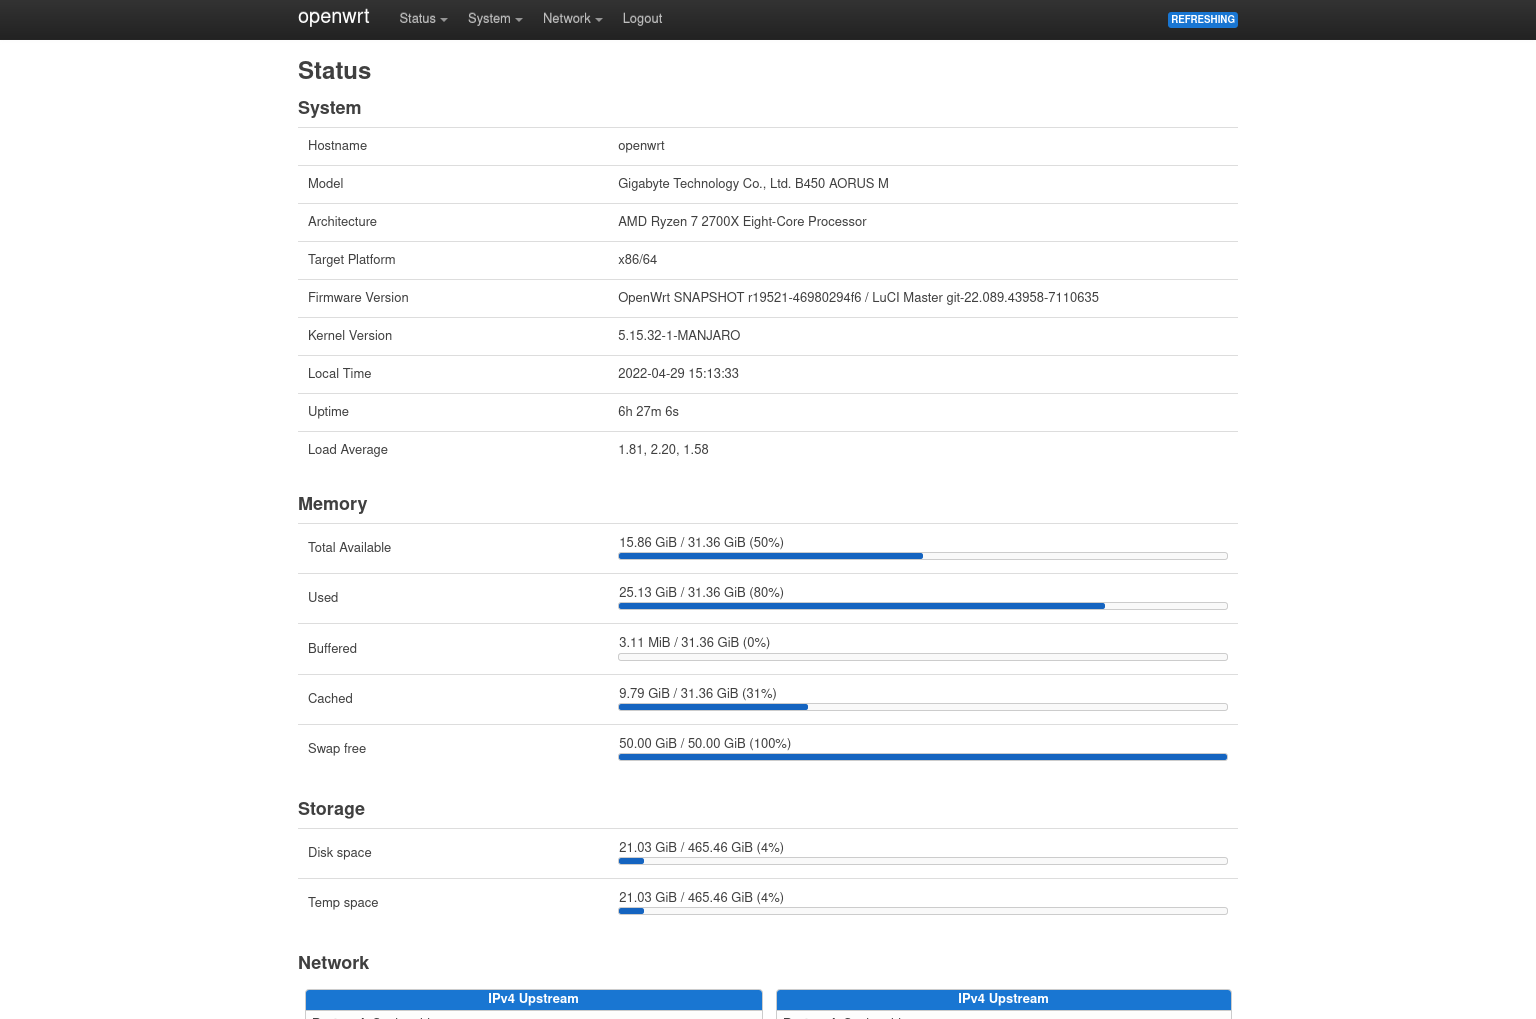
\includegraphics[height=0.65\linewidth]{immagini/LuCI_status}
        \caption{Status page}
        \label{fig:luci-status}
    \end{subfigure}%

    \medskip

    \begin{subfigure}{0.5\linewidth}
        \centering
        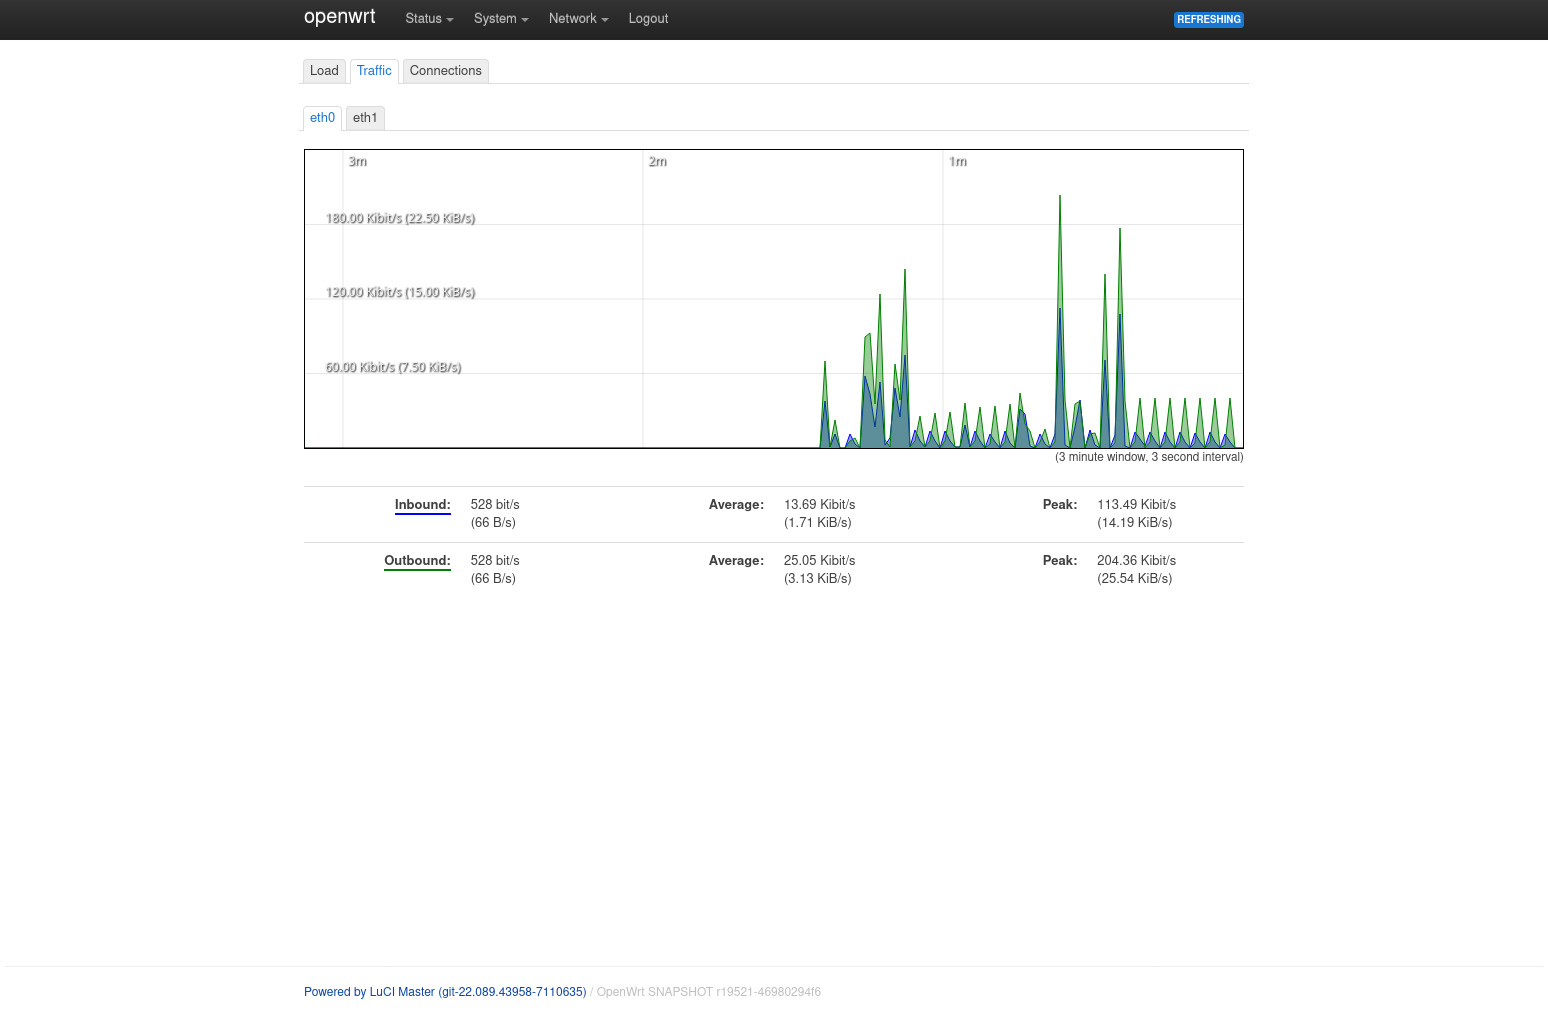
\includegraphics[height=0.65\linewidth]{immagini/LuCI_graphs}
        \caption{Graphs page}
        \label{fig:luci-graphs}
    \end{subfigure}%
    \hfill
    \begin{subfigure}{0.5\linewidth}
        \centering
        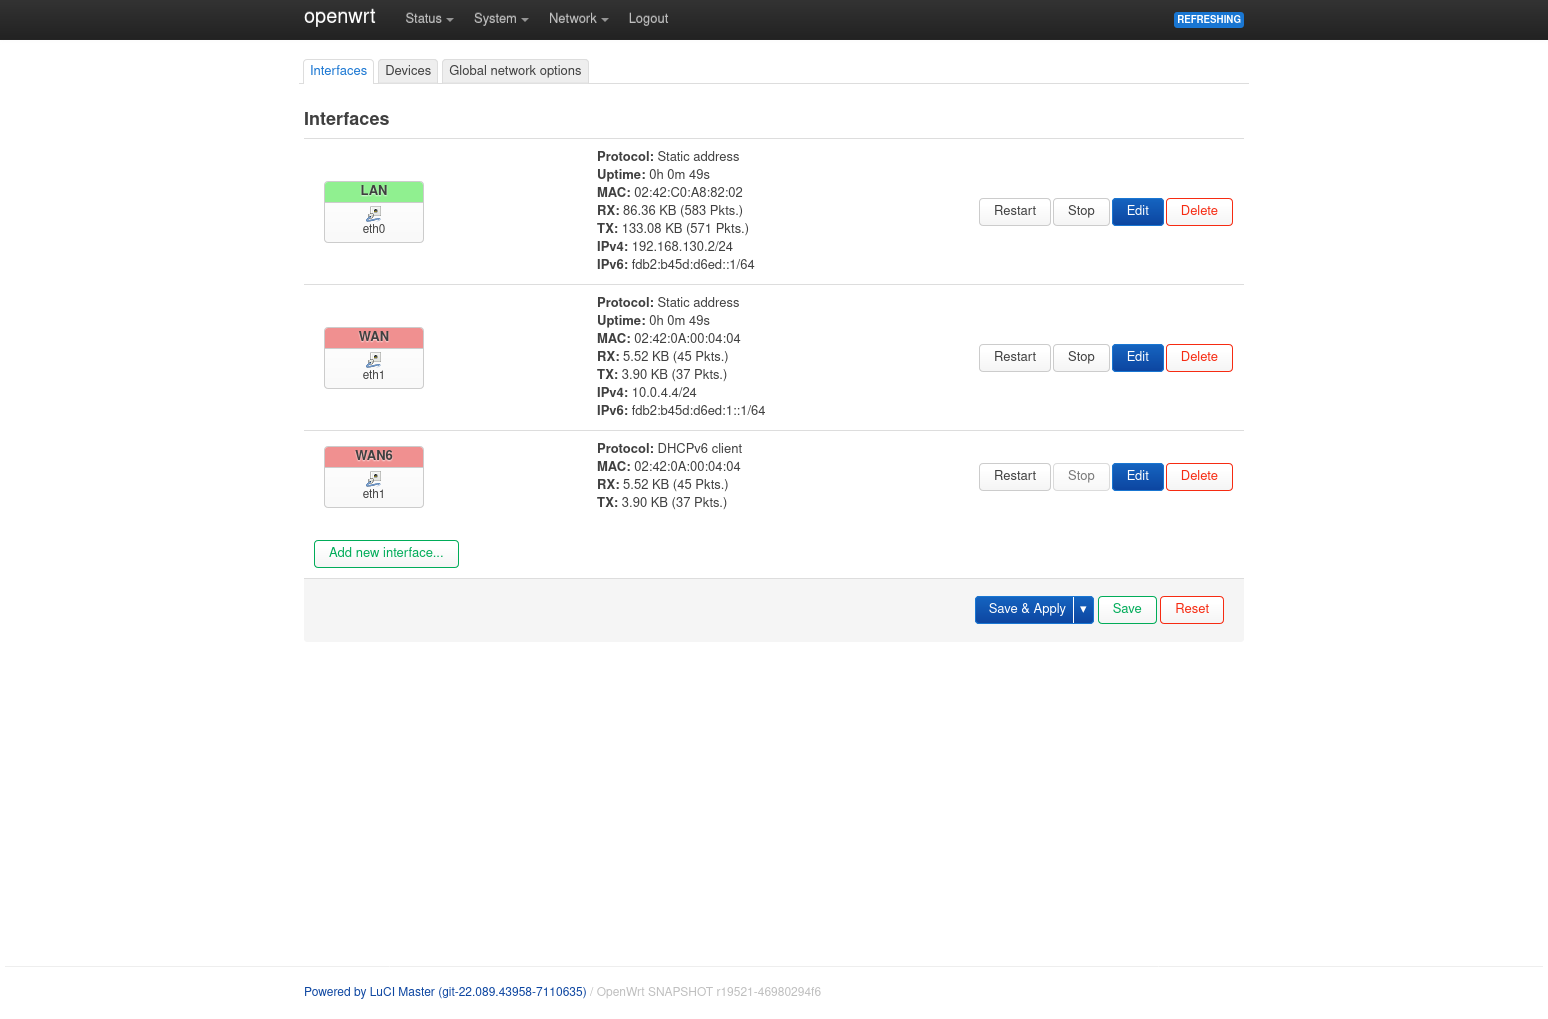
\includegraphics[height=0.65\linewidth]{immagini/LuCI_interfaces}
        \caption{Interfaces page}
        \label{fig:luci-interfaces}
    \end{subfigure}%
    \caption{Interfaccia web LuCI}
\end{figure}


L'homepage, fig. \ref{fig:luci-status}, mostra un riepilogo dello stato del router, ad esempio sono presenti: informazioni sull'hardware, informazioni sulla memoria e storage, sono presenti inoltre informazioni riassuntive sulle interfacce di rete e sul \it{DHCP}.

L'interfaccia è estensiva e permette di configurare quasi ogni aspetto del funzionamento del router, compreso il firewall, il \it{DHCP}, i processi in esecuzione, etc. 




